%+-------------------------------------------------------
%| CGAL Manual : arr.tex
%|
%| Soon to be split into User and Reference Manuals
%+--------------------------------------------------------
%| update log
%|
%|  1 Jun 2003  - Ron Wein
%|    Some updates and fixes.
%|
%| 21 Jun 2000  - Shai Hirsch
%|    arr_ref.tex was cut into an independent file.
%|
%| 04 May 2000  - Shai Hirsch
%|    Splitting into user and reference manual parts. Using new cc macros.
%|
%| 31 Mar 2000  - Shai Hirsch, 
%|    Changes for the 31/3/2000 deadline (differing user and ref.)
%|
%| Version  1.0 - Iddo Hanniel
%|    
%--------------------------------------------------------

%\maketitle


\section{Introduction}

Given a collection ${\mathcal C}$ of (possibly intersecting and not 
necessarily  $x$-monotone) curves in the plane, the planar arrangement of 
${\mathcal C}$ is the subdivision the curves of ${\mathcal C}$ induce on
the plane into zero-dimensional, one-dimensional and two-dimensional cells,
called {\emph vertices}, {\emph edges} and {\emph faces} respectively.

\section{Software Design}
 
The class \ccc{Arrangement_2<Dcel,Traits,Base_node>} is a data
structure for maintaining 2D arrangements. The data structure
maintains a planar map and curve hierarchy trees. There is a curve
tree for each curve inserted into the arrangement (see below). The
underlying combinatorial structure is determined by the
\ccc{Dcel} template parameter, which should be a model of the
\ccc{ArrangementDcel_2} concept. The family of curves of the
arrangement is determined by the \ccc{Traits} template parameter which
should be a model of the \ccc{ArrangementTraits_2} concept. The
\ccc{Base_node} template parameter defines the attributes associated
with each tree node of the hierarchy tree.

The \ccc{Arrangement} package is based on the \ccc{Planar Map with 
Intersections} package (see Chapter~\ref{I1_ChapterPmwx}). That is, given
a collection ${\mathcal C}$, we construct a collection 
${\mathcal C}''$ in two steps: First we decompose each curve in 
${\mathcal C}$ into maximal $x$-monotone curves, thus obtaining the 
collection ${\mathcal C}'$. We then decompose each curve in ${\mathcal C}'$ 
into maximal connected pieces not intersecting any other curve in 
${\mathcal C}'$. This way we obtain the collection ${\mathcal C}''$ of 
$x$-monotone, pairwise interior-disjoint curves.
The {\em arrangement} of the curves in $C$ is the
{\it planar map} (see Chapter~\ref{I1_ChapterPlanarMap})
induced by the curves in $C''$.

\paragraph{Curve Hierarchy Tree:} When constructing the arrangement of a
collection of curves ${\mathcal C}$, we decompose each curve $c \in 
{\mathcal C}$ in two steps: First we decompose it into maximal $x$-monotone 
curves, thus obtaining a set of curves $C'$. We then decompose each curve 
in $C'$ into maximal connected pieces not intersecting any other curve in 
${\mathcal C}$, obtaining the set $C''$.

We regard these sets $C'$, $C''$ as levels in a hierarchy of curves where the 
union of the subcurves in each level is the original curve $c$. We store these
sets in a special structure --- a {\em hierarchy tree}. This structure 
usually consists of three levels, although in some cases they can consist 
of less (e.g., when inserting an $x$-monotone curve) or more (when the users 
define their own {\em split functions} see Section~\ref{ssec:example4}). 
The levels are:
\begin{itemize}
\item Curve node level: the root of the tree --- holds the original curve $c$.
\item Subcurve node level: inner nodes of the tree --- hold decomposed
subcurves of the original curve. In the default mode these are $x$-monotone 
curves (that is, these nodes correspond to the sub-curves of $C'$).
\item Edge node level: leaves of the tree --- hold the curves corresponding to
the edges of the planar map induced by the arrangement (usually these nodes 
correspond to the sub-curves of $C''$). \newline
These nodes will be built only in {\em update mode} (by default the 
arrangement is in update mode).
\end{itemize}

Figure~\ref{fig:hierarchy} shows an example of a simple arrangement and its 
corresponding curve hierarchy.

%\vspace{-0.3cm}

\begin{figure}
\begin{ccTexOnly}
{\centerline {\includegraphics{Arrangement_2/arr_hier.ps}}}
\end{ccTexOnly}
\caption{A simple arrangement of two polylines, and its corresponding
hierarchy tree (the edges of the arrangement are numbered according to
their order in the tree).\label{fig:hierarchy}}
\begin{ccHtmlOnly}
<P>
<center><img border=0 src="./arr_hier.gif" alt=" ">
<!--
<br>
A simple arrangement of two polylines, and its corresponding hierarchy tree
(the edges of the arrangement are numbered according to their order
in the tree).
-->
</center>
\end{ccHtmlOnly}
\end{figure}

The hierarchy tree enables us to intersect the curves without loss of
information. The original curve and the intermediate subcurves are stored
in the tree and the user can traverse them. Furthermore, users can
define their own hierarchy by passing their own intersection sequence.
This can be of use in some applications. For example, in an arrangement
of spline curves the users might want to intersect a curve in the
junction points before making the curve $x$-monotone. 

\paragraph{Degeneracies} Like the planar map package (see
Chapter~\ref{I1_ChapterPlanarMap}), the arrangement package can deal
with $x$-degenerate input (including vertical segments). However,
while in the planar map the input curves were assumed to be
$x$-monotone and non-intersecting in their interiors, there are no
such assumptions in the arrangement. A non $x$-monotone curve is
partitioned into $x$-monotone subcurves, and curves are intersected in
their points of intersection with other points before they are
inserted into the map. Furthermore, overlapping curves are
supported. If two curves overlap the traits intersection function
returns the two endpoints of the common part. Circulators of the
\ccc{Overlap_circulator} type (of 
\ccc{Arrangement_2<Dcel,Traits,Base_node>}) enables to traverse all
overlapping \ccc{edge_nodes} that correspond to the same pair of
halfedges in the map.

\paragraph{I/O functions:}
I/O functions for reading a saved arrangement from the standard input, 
writing it to the standard output or drawing it to a graphic stream are 
also provided.
Users of I/O functions for the arrangement package are required to define I/O 
operators for the curves defined in their \ccc{Traits} classes.

\paragraph{Update Mode:} For some algorithms, it is not necessary to build
the whole planar map induced by the arrangement. For example, the lower
envelope of an arrangement of $x$-monotone curves that intersect
each other at most a fixed constant number of $s$ times,
can be found in near linear time \cite{sa-dsstg-95, h-a-97}
even if
the complexity of the planar map induced by it is quadratic.
Therefore, building the planar map induced by the arrangement is not
always desired. The users can therefore disable (or postpone) the building
of the planar map. This is done by disabling the {\it update mode}
using the \ccc{set_update(bool)} member function. When update mode is
set to \ccc{true}, the planar map is updated --- this is the
default situation. 
When update mode is set to \ccc{false}, the hierarchy tree is built without
its \ccc{Edge_level}, and the curves are not inserted into the planar map.

%******************************************************************************

%\section{Example Programs}
%---------------------------------------------------
\section{Segment Arrangements}

The second template parameter of the arrangement class determines the
so-called geometry of the arrangement, that is the family of curves we
want to deal with. In order to deal with line segments we simply plug
in on of the two segment traits classes supplied.

The \ccc{Arr_segment_traits_2<Kernel>} class is generic and allows
flexibility in determining the kernel which is used. It makes intensive
use of the kernel, since it support almost all the operations needed by the
arrangement package. The \ccc{Arr_segment_cached_traits_2<Kernel>} class
stores some additional cached information with each segment curve. Choosing
to work with this traits class means a little extra memory consumption, 
however it usually speeds up the construction time of the arrangement.

\subsection{Example of an Arrangement of Segments}
The following example demonstrates the construction of an $X$-shaped
arrangement out of two segments.  After the construction we traverse
the edges of the arrangement in the order defined by the original
segments.

The four numbers on each output lines is a representation of a segment.
The first two numbers are the $x$ and $y$ coordinates of the first endpoint.
The other two numbers are of the second endpoint. The way a curve is
printed depends on the the output operator implemented for it.

\ccIncludeExampleCode{Arrangement_2/example1.C}

The output of the program looks like this:
\begin{verbatim}
Curve level:
0 0 1 1
Edge level:
0 0 0.5 0.5
0.5 0.5 1 1

Curve level:
0 1 1 0
Edge level:
0 1 0.5 0.5
0.5 0.5 1 0
\end{verbatim}

\subsection{Example of Overlapping Segments}
\label{ssec:example2}
The following example demonstrates the construction of an
arrangement out of two overlapping segments --- $(0,0)-(2,2)$
and $(1,1)-(3,3)$.
After the insertion of the segments we
traverse the halfedges
of the arrangement and count the overlapping curves.
This is done using the \ccc{overlap_edges()} member function that returns an
\ccc{Overlap_circulator}. With it we can circulate
over all the edge nodes that correspond to the halfedge.

\ccIncludeExampleCode{Arrangement_2/example2.C}

The output of the program looks like this:
\begin{verbatim}
Edge 0 0 1 1 is covered by a single edge.
Edge 1 1 2 2 is covered by 2 edges.
Edge 2 2 3 3 is covered by a single edge.
\end{verbatim}

\section{Polyline Arrangements}

The \ccc{Arr_polyline_traits_2<Segment_traits>} class can be used to 
handle arrangements of polylines (a.k.a. poly-segment). A polyline can be
created from any range of points, where the $i$th and $(i+1)$st points 
in the range represent the endpoints of the $i$th segment of the polyline.
The polyline traits class is templated with another traits class that supports
the basic operations on segments. 

\subsection{Example of a Polyline Arrangement}
\label{ssec:example10}
The following example demonstrates the use of the polyline traits.
Observe that a polyline curve is constructed from a standard STL vector
of points.

Note that a polyline point is not necessarily a vertex of the arrangement 
(that is, of the underlying Planar Map) and an edge of the Planar Map need 
not be a segment. The edges are only required to be x-monotone and pairwise 
disjoint. In the example below point (150, 50) is not a vertex of the planar 
map. The polyline to which it belongs is an edge of the planar map.

 However, one might expect the planar map (or rather the edge level of the 
arrangement) to be made of segments alone. In such cases the user can define 
additional level of hierarchies, as will be shown in the example in 
Section~\ref{ssec:example4}.

\ccIncludeExampleCode{Arrangement_2/example10.C}

\section{Arrangements of Conic Arcs}

The \ccc{Arr_conic_traits_2<Int_kernel, Alg_kernel>} class can be used for
constructing arrangement of bounded segments of algebraic curves of degree 2
(conic curves).
That is, it supports the construction of the arrangement of any 
collection of elliptic arcs (a full ellipse or a circle may also be considered
as a conic arc), hyperbolic arcs, parabolic arcs and also line segments.
The template has two template parameters:
\begin{itemize}
\item The first template parameter, \ccc{Int_kernel}, is a geometric kernel
with an unbounded integer number-type (i.e.~\ccc{Int_kernel::FT}, or 
\ccc{CfNT} for short, should be an unbounded integer), that represents the
coefficients of the conic curves. The kernel \ccStyle{Cartesian<CORE::BigInt>}
is the most suitable choice for this parameter.
\item The second parameter, \ccc{Alg_kernel}, is a geometric kernel whose 
number type (\ccc{Alg_kernel::FT}, or \ccc{CoNT} for short) supports exact
operations: In addition to the arithmetic operations, it must support the
square-root operation in an exact manner, as well as the extraction of the
$k$th-largest root of a given polynomial with integral coefficients.
\ccc{CoNT} should be constructible from a \ccc{CfNT}, and it is used to
represent the coordinates of the arrangement vertices (which are in general
irrational algebraic numbers). At current, the \ccStyle{CORE:Expr} is the only
number type that fills all the requirements above and must be the number
type of \ccc{Alg_kernel}.
\end{itemize}

\subsection{Example of an Arrangement of Circular Arcs}
\label{ssec:example3}
The following example demonstrates the use of the conic traits for 
constructing a simple arrangement of two circles. The arrangement created 
by this example is depicted in Figure~\ref{fig:circles}. Note that each
circle is divided to an upper half and a lower half, both are $x$-monotone:
The result of ray-shooting operation from $(-1,0)$ upward exemplifies this, 
since it returns a circular arcs whose end-points are $(3,4)$ and $(-5,0)$.

\begin{figure}[h]
\begin{ccTexOnly}
{\centerline {\includegraphics{Arrangement_2/arr_circ.ps}}}
\end{ccTexOnly}
\caption{The arrangement generated by the example program.\label{fig:circles}}
\begin{ccHtmlOnly}
<P>
<center><img border=0 src="./arr_circ.gif" alt=" ">
<!-- <br>The arrangement generated by the example program. -->
</center>
\end{ccHtmlOnly}
\end{figure}

\ccIncludeExampleCode{Arrangement_2/example3.C}

\subsection{Example of an Arrangement of Mixed Conic Arcs}
\label{ssec:example13}

The following example demonstrates the construction of an arrangement
of various conic arcs of mixed types. The input \ccc{Curve_2} objects are
created in a way that makes use of most available constructors for conic
arcs.

The arrangement created by this example is depicted in 
Figure~\ref{fig:conics}. The program outputs the number of vertices, edges and
faces in the resulting arrangement, and the correctness of these figures can
be easily verified by counting them in this figure: Notice that arrangement
vertices may be original endpoints of the input curves, intersection points
of two (or more) curves or points where the tangent to the curve is a vertical
line.

\begin{figure}[h]
\begin{ccTexOnly}
{\centerline {\includegraphics{Arrangement_2/arr_conics.ps}}}
\end{ccTexOnly}
\caption{The arrangement of conic arcs generated by the example program.
The coordinates of the input endpoints are also shown.
\label{fig:conics}}
\begin{ccHtmlOnly}
<P>
<center><img border=0 src="./arr_conics.gif" alt=" ">
<!-- <br>The arrangement generated of conic arcs by the example program. -->
</center>
\end{ccHtmlOnly}
\end{figure}

\ccIncludeExampleCode{Arrangement_2/example13.C}

The output of the program looks like this:
\begin{verbatim}
Number of vertices: 19
Number of edges: 23
Number of faces: 6
\end{verbatim}

\begin{ccAdvanced}
\section{User-defined Hierarchy}

The default hierarchy structure can be extended to include more levels
according to user defined split functions.

\subsection{Example of a User-defined Hierarchy}
\label{ssec:example4}

The following example demonstrates the construction of an
arrangement of two segments, using a user-defined
hierarchy.
We use a simple split function that splits a segment in its middle
point. We insert the first segment using the user-defined function
and the second segment with the regular function.

\ccIncludeExampleCode{Arrangement_2/example4.C}

The output of the program looks like this:
\begin{verbatim}
Curve level:
0 0 6 6
Edge level:
0 0 3 3
3 3 4 4
4 4 6 6

Curve level:
0 4 6 4
Edge level:
0 4 4 4
4 4 6 4
\end{verbatim}

\end{ccAdvanced}


\begin{ccAdvanced}

\subsection{Example of a User-defined Hierarchy with Function Objects}
\label{ssec:example5}

The following example demonstrates the use of a function object in
a user-defined hierarchy. We define a base class for the function objects
with a virtual \ccc{operator()}, that the function objects override (this
kind of pattern is sometimes called an \ccc{Action} class
(see for example \cite[Chapter~25.5]{cgal:s-cpl-97}). This enables us to
use an inner state in our function as is done in the example.

In the example we define two levels of a hierarchy. The first level
splits the inserted segment in the middle. The second layer splits every
curve of the first layer in a ratio of $1/3 : 2/3$. Therefore, after
an insertion of the segment $(0,0) - (6,6)$
we will have four edges (eight halfedges)
inside the arrangement, corresponding to the segments: $(0,0) - (1,1)$,
$(1,1) - (3,3)$, $(3,3) - (4,4)$ and $(4,4) - (6,6)$.

%\ccIncludeExampleCode{example5.C}
\ccIncludeExampleCode{Arrangement_2/example5.C}

\end{ccAdvanced}

\begin{ccAdvanced}
\subsection{I/O functions}
The \ccc{Arrangement} package supports I/O functions, which include reading 
an arrangement representation from 
the standard input or writing it to the standard output, 
and also sending an arrangement to a graphic stream.

As already mentioned at chapter \ccRefPage{Pm_Ref_intro}, the motivation for 
using I/O functions is not only to be able to draw the arrangement 
to a window for instance, but also to be capable to save an arrangement 
in a text file by writing it and reloading it from a text file by reading it. 
 
Reading an arrangement from the standard input or printing it to the
standard output may be done simply with the \ccc{Extractor} (\ccc{ >>
}) and \ccc{Insertor} (\ccc{ << }) operators defined for
\ccc{Arrangement_2}, respectively. 

\ccInclude{CGAL/IO/Arr_iostream.h}

The ability of sending the \ccc{Arrangement} 
into a graphic stream as \ccStyle{leda_window}, Postscript file or
Geomview is also provided, users simply have to apply the Insertor
operator on the graphic stream and their arrangement instance.

Users of I/O functions for the arrangement package are required to define I/O 
operators for the curves defined in their \ccc{Traits} classes. 
When using \ccc{Traits} classes in which this operators are already defined 
(as \ccc{Segment Traits}) the operator definition is not obligated, 
however using \ccc{Traits} classes as the \ccc{Conic Traits} will force 
the users to define I/O operators on their conic curve.

The \ccc{Arrangement} class data consists of the induced planar map and the 
obtained hierarchy tree. Hence, the data sent to the output stream or 
read from an input stream should contain both parts. 

The format of the planar map part is as specified in the Planar Map 
reference pages (\ccRefPage{Pm_Ref_intro}). 
The format of the hierarchy tree is specified below.

The format of the output file is defined in a way the reading function 
will construct the arrangement efficiently. 
The induced planar map is constructed efficiently as specified in the Planar 
Map reference pages (\ccRefPage{Pm_Ref_intro}), and the hierarchy tree is also 
constructed efficiently by directly accessing its parts and updating them. 
When constructing an arrangement from an input stream, no use of its 
insertion functions is performed.
 
Consequently, the reading function constructs the arrangement very 
efficiently, and hence users who would like to save their arrangement and 
reload it have to construct their  arrangement by the insertion functions 
only once. After saving the arrangement to a text file it can be reloaded 
very efficiently when needed, instead of constructing it from scratch.

When users would like to read their arrangement from the standard input or 
print it into the standard output, they may simply use the \ccc{Extractor} 
(\ccc{ >> }) and \ccc{Insertor} (\ccc{ << }) operators defined for 
\ccc{Arrangement} respectively. 
If users add attributes to their arrangement components, reading (resp. 
writing) arrangement would be done by inheriting the class 
\ccStyle{Arr_file_scanner}  (resp. \ccStyle{Arr_file_writer} ) 
and overriding all the relevant function for scanning (resp. writing) the 
arrangement components. After the definition of the inherited class users 
have to call the function \ccStyle{read} of \ccc{Arrangement} (resp. the 
global function \ccStyle{write_arr} ) with the inherited class as a parameter.
The ability of sending the \ccc{Arrangement} into a graphic stream as 
\ccStyle{leda_window}, Postscript file or Geomview is also provided, 
users simply have to use the Insertor operator operated on the graphic 
stream and their arrangement. When users would like to add attributes to 
their arrangement components and send their arrangement to a graphic stream, 
they have to inherit the class \ccStyle{Pm_drawer} and then call the global 
function \ccStyle{draw_pm} with this class and their arrangement as parameters.
The function  \ccStyle{Pm_drawer} is used both for \ccc{Planar map} and 
\ccc{Arrangement}, since drawing an arrangement is defined as drawing only 
its planar map part.

\paragraph{Format}
\ccRefLabel{Arr_IO_format}
As mentioned above, the format of the planar map part is as specified 
in the Planar Map reference pages (\ccRefPage{Pm_Ref_intro}). 
Here, we are representing the format of the hierarchy tree.

Generally, the format represents the curve nodes list of the 
\ccc{arrangement}. Each component of one curve node is compound from all the 
subcurves and edge nodes this curve node contains. This data is associative 
with geometric information and some topological information in order to be 
able to update the hierarchy tree efficiently. 

The format is detailed below:

\begin{enumerate}
    \item The data begins with a line of one integer specifying the number 
    of curve nodes the hierarchy tree has.
    \item The list of curve nodes: 
    each curve node has the following format:
    \begin{enumerate}
        \item Its associative curve.
        \item An integer specifying the number of levels the curve node has.
        \item The list of all subcurves levels. Each described level goes as 
              follows:
        \begin{enumerate}
            \item An integer specifying the number of subcurve nodes in the 
                  current level.
            \item List of subcurve nodes belong to the current level. 
            Each subcurve consist of the following:
            \begin{enumerate}
                \item Pointers to subcurves (edge nodes, if the next level 
                      is the last) 
                      of lower level which are given as the begin and past 
                      end indices of children subcurve nodes (edge nodes).
                \item The curve associative with the subcurve node.
            \end{enumerate}
        \end{enumerate}
        \item An integer specifying the number of edge nodes.
        \item List of edge nodes. Each described edge node goes as follows:
        \begin{enumerate}
            \item A pointer to an overlapping edge node.
            This pointer is represented by two indices, the first is an index 
            to a curve node 
            and the second is an index to an edge node defined in that curve 
            node.
            \item An index to the associated halfedge.
            \item The associated curve.
        \end{enumerate}    
    \end{enumerate}
\end{enumerate}

Other rules concerning the format are detailed in the Planar Map 
reference pages (\ccRefPage{Pm_Ref_intro}).

\subsubsection{Example of Usage of the I/O Functions}
\label{ARR_sec:example11}

The input of the program is a text file presenting the \ccc{Arrangement}:
\ccIncludeExampleCode{Arrangement_2/example11.cin}

The example above presents an arrangement containing two segments that 
intersect in their interior. The segments are $(0,0) -- (1,1)$ and $(0,1) --
(1,0)$.  The \ccc{Arrangement} instance that was used to produce this example 
was templated  with the \ccStyle{Arr_segment_traits_2} class, which was 
templated with the representation class \ccStyle{Cartesian<Quotient<int> >}.

The first part of the input represents the planar map our arrangement 
contains, and hence its format is identical with \ccRefPage{Pm_IO_format}. 
It can be seen that the planar map described here represents all the vertices 
and halfedges obtained by the disjoint subcurves of the arrangement.

The next part of the input file presents the hierarchy tree of our 
arrangement. This presentation begins with the number 2, indicating there are 
two curve nodes in our arrangement. The list of curve nodes follows.
The first curve node begins with its associated curve $(0,0) -- (1,1)$, 
it has 0 levels since it does not contain any subcurve nodes (only curve 
nodes and edge nodes). 
The number of edge nodes the curve $(0,0) -- (1,1)$ induces is two, 
and the curves these two edge nodes are associated with are 
$(0,0) -- (1/2,1/2)$ and $(1/2,1/2) -- (1,1)$ respectively. 
The indices of each edge node to an overlapping edge node point to the edge 
node itself since there are no overlapping in the input file. 
Finally, the indices of the halfedge indicates the halfedge our edge node is 
associated with. 
For example, the first edge node induced by the curve $(0,0) -- (1,1)$ is 
associated  with the first halfedge presented in the halfedges list. The 
reader may verify that this halfedge holds the same curve the edge node holds.

The current format may not be comfortable for a user to read, because the 
usage of indices. There is a possibility to define a verbose format which 
contains instead of indices, the components themselves, and hence the user 
has the option to have a format which is easy for human to read.
This format cannot be scanned by the reading functions of \ccc {Arrangement}.

\ccIncludeExampleCode{Arrangement_2/example11.C}

The output is the \ccc{Arrangement} written in both formats, non verbose and 
verbose. 
\ccIncludeExampleCode{Arrangement_2/example11.cout}

For more examples see chapter \ccRefPage{Pm_Ref_intro}.

More details are given in sections
\ccc{Arr_file_scanner<Arrangement>}\lcTex{
   (\ccRefPage{CGAL::Arr_file_scanner<Arrangement>})}, 
\ccc{Arr_file_writer<Arrangement>}\lcTex{ 
   (\ccRefPage{CGAL::Arr_file_writer<Arrangement>})} 
\end{ccAdvanced}

% EOF ---------------------------------------------------------------------80










